\item En la figura \ref{fig:aspersor} se observa un aspersor de un solo brazo visto en planta. El mismo rota respecto del punto $O$ a velocidad constante $\omega$. El flujo de agua $Q$ ingresa desde un caño vertical a través de $O$. El torque resistente que se produce en el cojinete es $-T_O$. ¿Cual es la expresión que define la velocidad de rotación $\omega$?. En caso de que el aspersor tuviese cuatro brazos separados entre sí a 90$^\circ$, ¿cual es la expresión de la velocidad?, ¿y si existiesen infinitos brazos aspersores?

\begin{figure}[h!!!!]
\centering
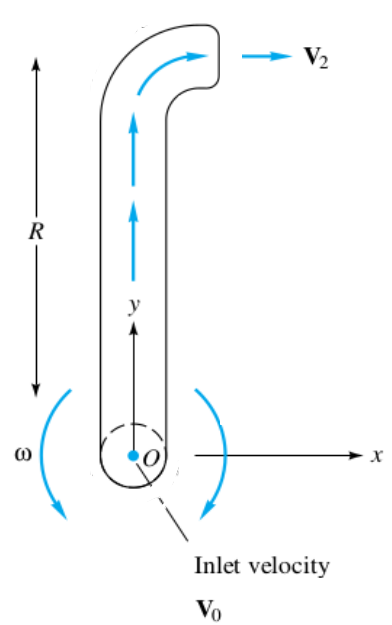
\includegraphics[width=0.3\textwidth]{aspersor.png}
\caption{Aspersor de un brazo}
\label{fig:aspersor}
\end{figure}

